\clearpage
\section{Quantum Random Number Generator}

\begin{tcolorbox}	
\begin{tabular}{p{2.75cm} p{0.2cm} p{10.5cm}} 	
\textbf{Students Name}  &:& Mariana Ramos (12/01/2018 - )\\
\textbf{Goal}          &:& Simulate and implement an experimental setup of a Quantum Random Number Generator.\\
\textbf{Directory}          &:& sdf/quantum\_random\_number\_generator.
\end{tabular}
\end{tcolorbox}

True random numbers are indispensable in the field of cryptography\cite{katsoprinakis2008quantum}. There are two approaches for random number generation: the pseudorandom generation which are based on an algorithm implemented on a computer, and the physical random generators which consist in measuring some physical observable with random behaviour. Since classical physics description is deterministic, all classical processes are in principle predictable. Therefore, a true random number generator must be based on a quantum process.\cite{Zeilinger}

In this chapter, it is presented the theoretical, the simulation and the experimental analysis of a quantum random generator based on the use of single photons linearly polarized at $45^{\circ}$.

\subsection{Theoretical Analysis}

One of the optical processes available as a source of randomness is the splitting of a polarized single photon beam. The principle of operation of the random generator is shown in figure \ref{qrng}. Each individual photon coming from the source is linearly polarized at $45^\circ$ and has equal probability of be found in the horizontal (H) or in the vertical (V) output of the PBS. Quantum theory estimates for both cases that the individual choices are truly random, independent one from each other , and with a probability of 1/2.

\begin{figure}[H]
    \centering
        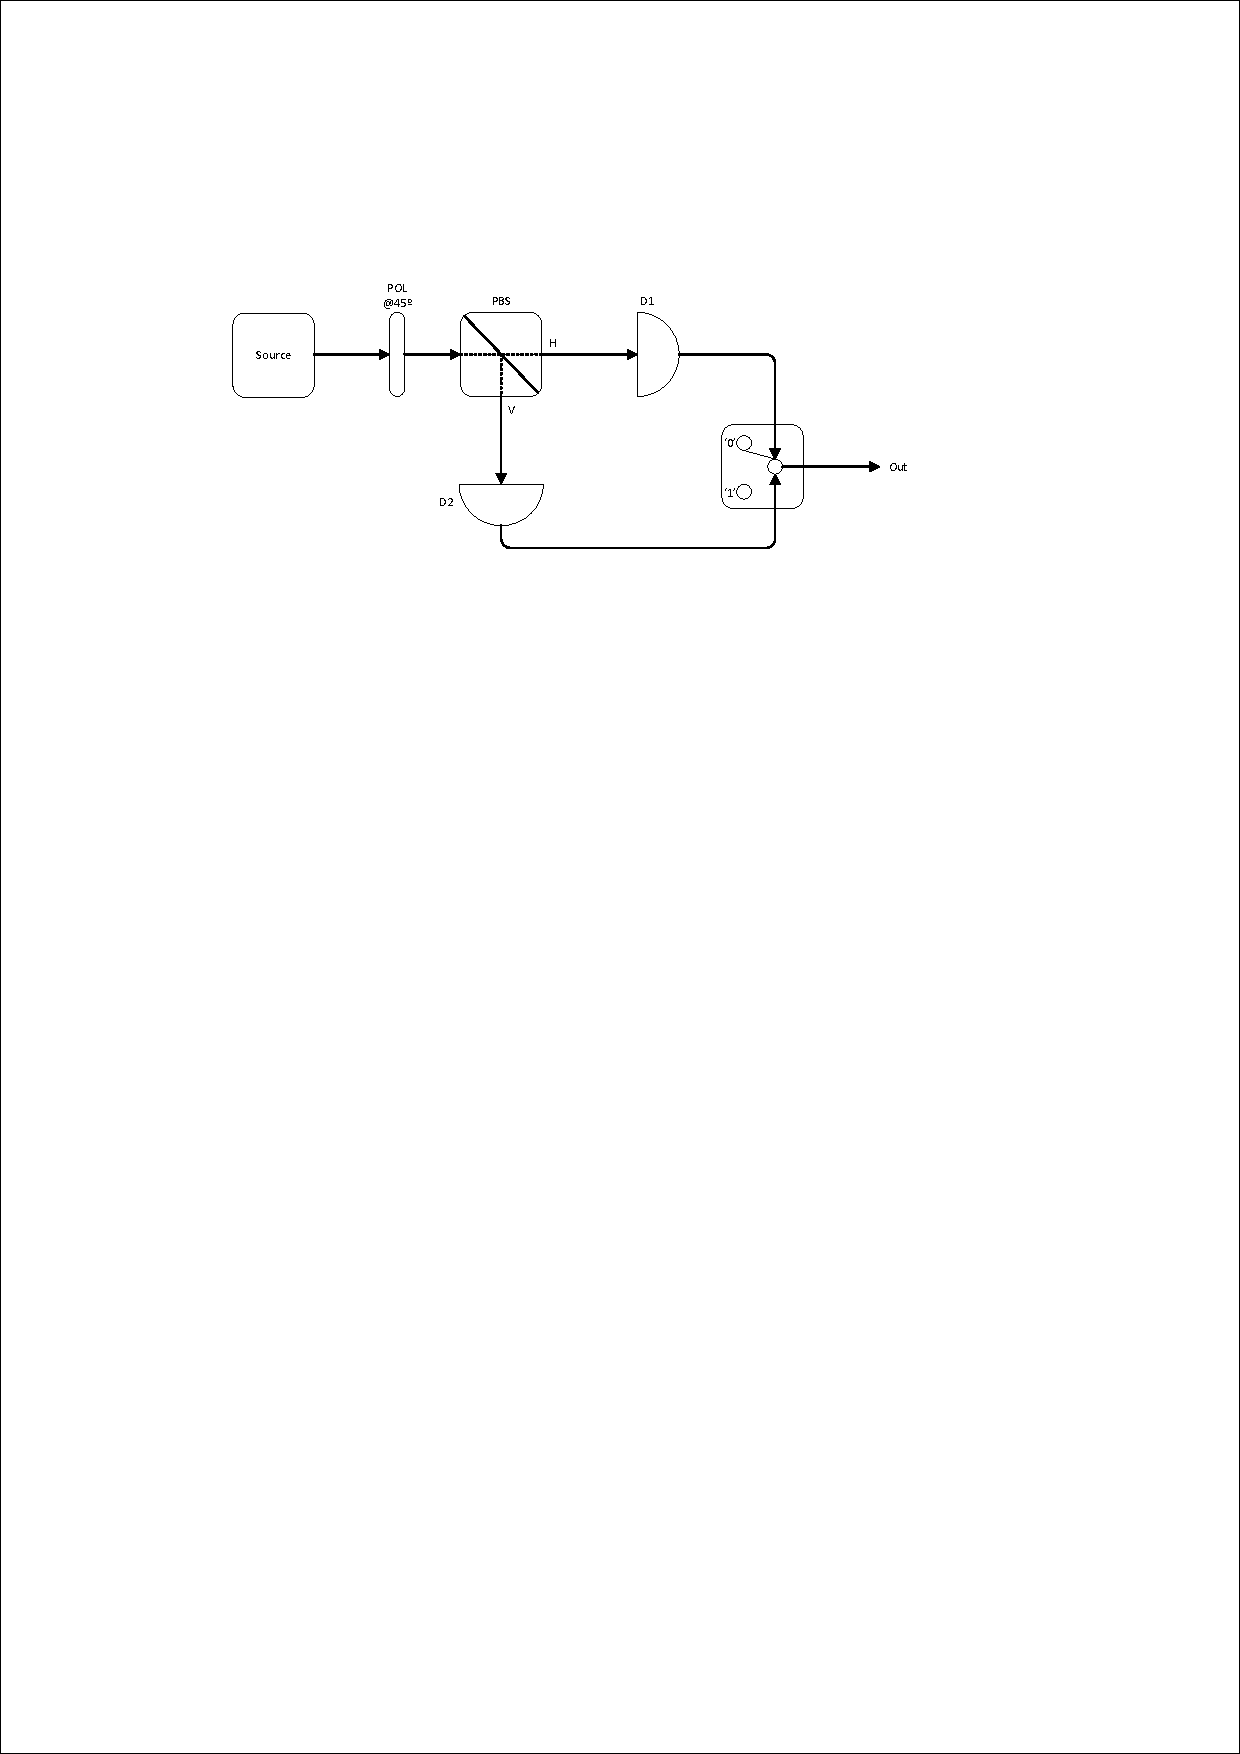
\includegraphics[clip, trim=3cm 20cm 5cm 5cm, width=1.00\textwidth]{./sdf/quantum_random_number_generator/figures/Random_Number_Generator.pdf}
    \caption{Source of randomness with a polarization beam splitter PBS where the incoming light is linearly polarized at $45^{\circ}$ with respect to the PBS. Figure adapted from \cite{Zeilinger}.}\label{qrng}
\end{figure}

From a classical approach, the information is stored as binary bits that can take the logical value '0' or '1'. From a quantum approach, the information can be stored in quantum bits or qubits for short. As a consequence of the superposition principle of quantum mechanics, qubits can not only represent the pure '0' or '1' states, but they can also represent a superposition of both. This way, qubits are governed by a quantum wave function $\psi$. Lets use the Dirac notation to represent the general state of the qubit:
\begin{equation}\label{eq:qubit}
  |\psi\rangle = C_0 |0\rangle + C_1 |1\rangle,
\end{equation}

and the normalization condition of $|\psi\rangle$ requires that $|C_0|^2+|C_1|^2=1$. This way, the relative proportion of each of the binary states on a qubit is governed by the amplitude coefficients $C_0$ and $C_1$. In the present example, we consider a linear polarization in which the two possible states are orthogonal, such that: $\langle 0|1 \rangle=0$. We define the $|0\rangle$ and $|1\rangle$ states to correspond to the horizontal and vertical polarization states, respectively:

\begin{eqnarray}
 %\nonumber % Remove numbering (before each equation)
  |\psi\rangle &=& C_0 |0\rangle+C_1 |1\rangle \\
             &=& C_0 |0^{\circ}\rangle + C_1 |90^{\circ}\rangle .
\end{eqnarray}

Amplitude coefficients $C_0$ and $C_1$ store the quantum information. Therefore, if one makes a measurement, the result will be '0' with probability $|C_0|^2$ or '1' with probability $|C_1|^2$.
Moreover, the state of a single photon can be also described by a wave function as a column vector:

\begin{equation}\label{eq:wavefvector}
  |\psi\rangle = \binom{C_0}{C_1},
\end{equation}
which will be used in simulation analysis.

\begin{figure}[h]
    \centering
        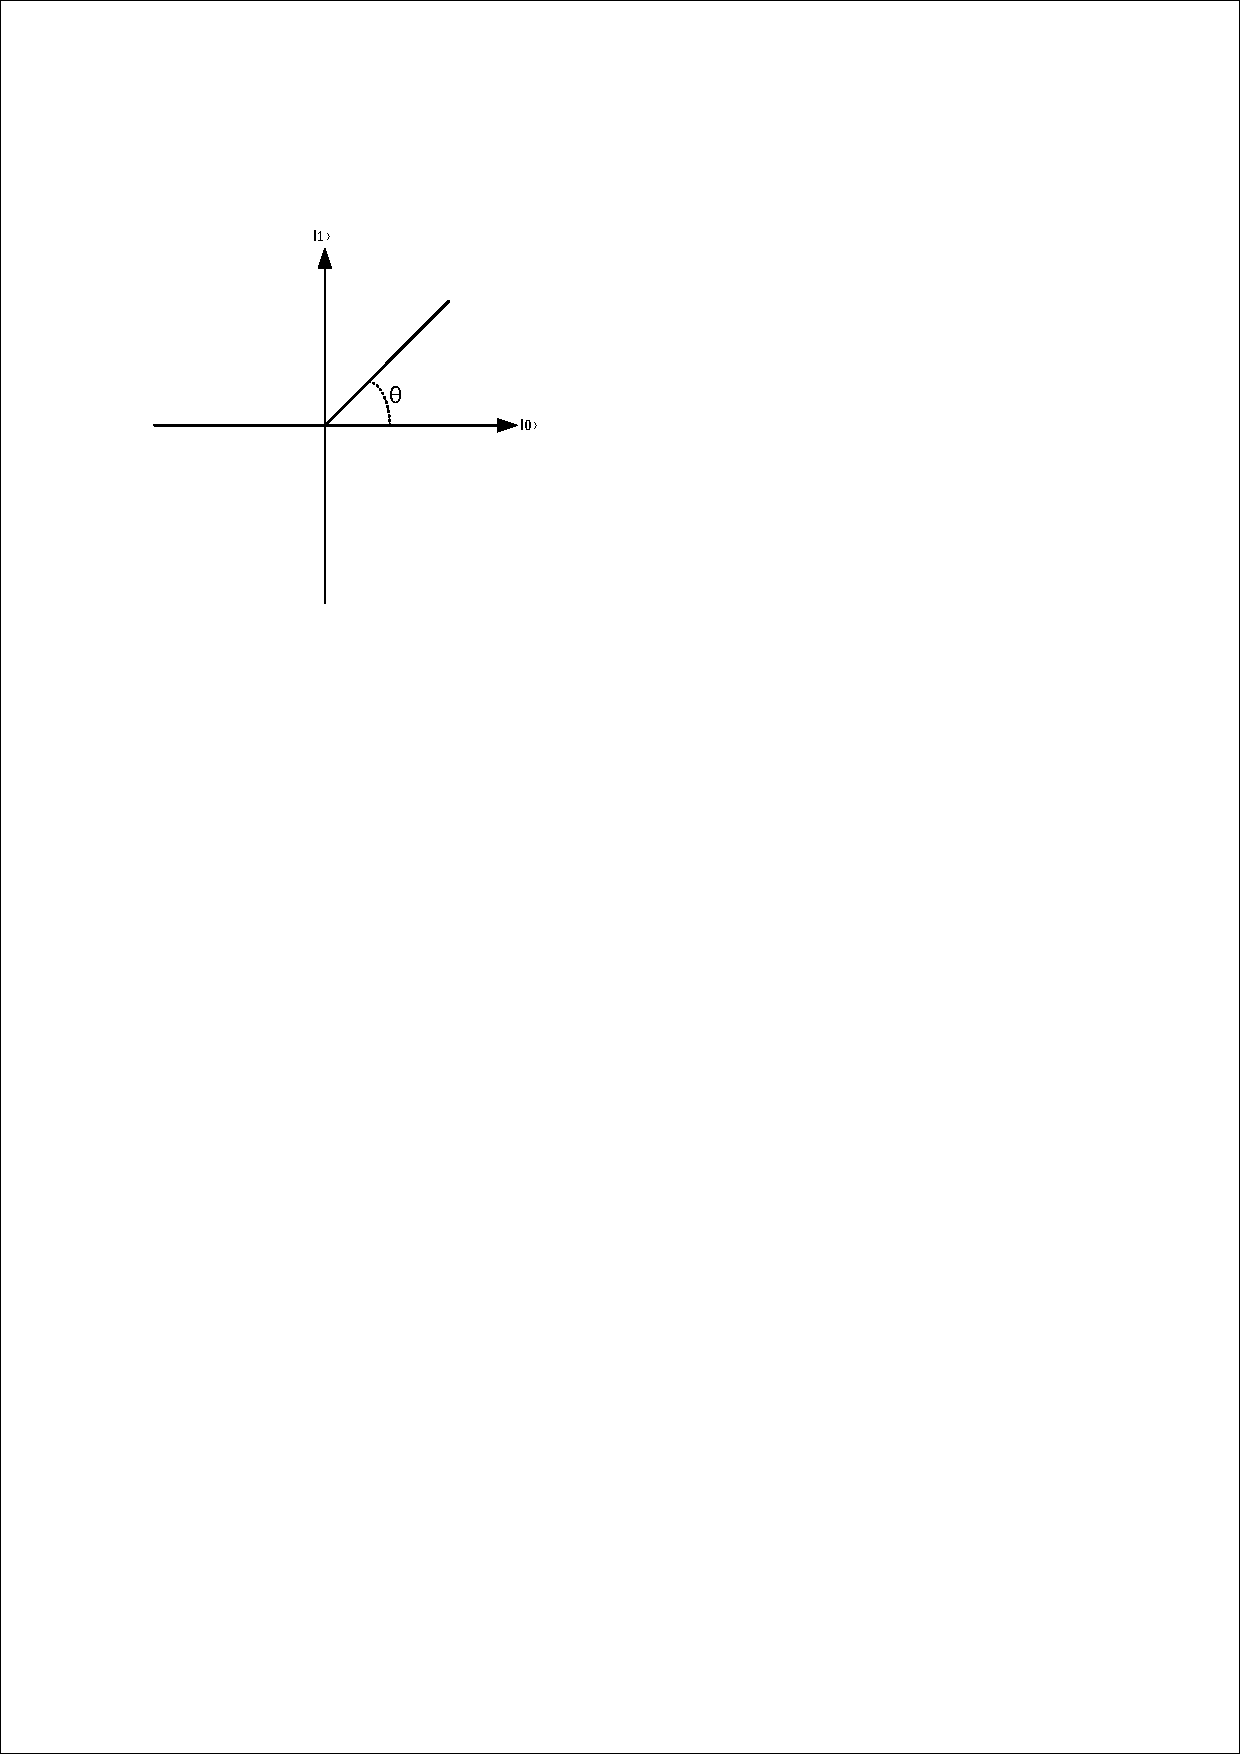
\includegraphics[clip, trim=3cm 20cm 12cm 3cm, height=6cm]{./sdf/quantum_random_number_generator/figures/axis_states.pdf}
    \caption{Representation of polarization states of a qubit in a bi-dimensional space.}\label{fig:stateaxis}
\end{figure}

As one can see in figure \ref{fig:stateaxis} the amplitude coefficients can be written as a function of $\theta$:
\begin{eqnarray}
% \nonumber % Remove numbering (before each equation)
  C_0 &=& cos(\theta) \\
  C_1 &=& sin(\theta).
\end{eqnarray}

According with the setup presented in figure \ref{qrng} and considering the polarization angle $\theta = 45^{\circ}$, the single photon has the probability of reach \textbf{D1} and outputs a "$0$" is equals to $|cos(\theta)|^2$ and the probability of reach \textbf{D2} and outputs a "$1$" is equals to $|sin(\theta)|^2$, which in the case $\theta = 45^{\circ}$ both have the same value equals to $0.5$.

\subsection{Simulation Analysis}
The simulation diagram of the setup described in the previous section is presented in figure \ref{sim_qrng}. The linear polarizer has an input control signal (S1) which allows to change the rotation angle. Nevertheless, the only purpose is to generate a time and amplitude continuous real signal with the value of the rotation angle in degrees. In addition, the photons are generated by single photon source block at a rate defined by the clock rate. At the end of the simulation there is a circuit decision block which will outputs a binary signal with value "$0$" \space if the detector at the end of the horizontal path clicks or "$1$" \space if the detector at the end of the vertical path clicks.

\begin{figure}[h]
    \centering
        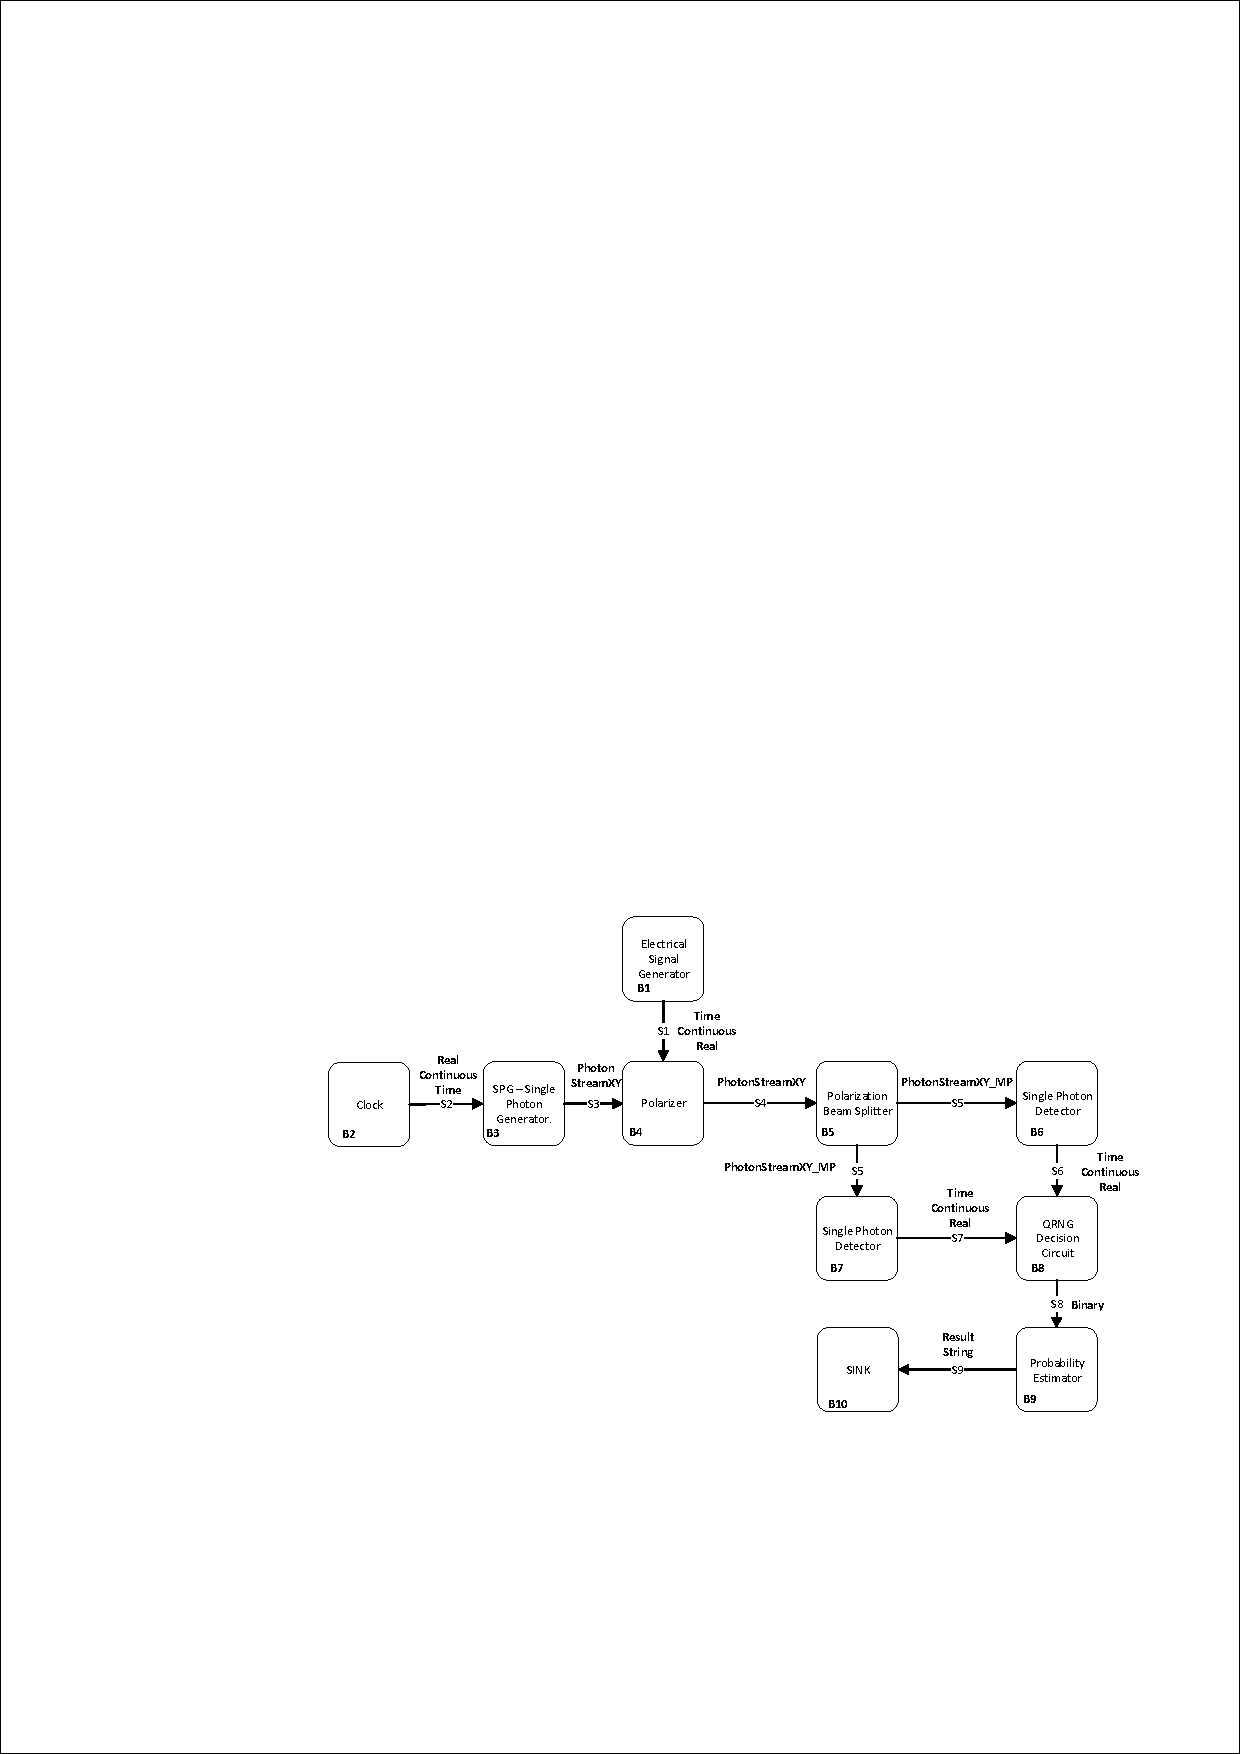
\includegraphics[clip, trim=5cm 5cm 0.5cm 15cm, width=1.00\textwidth]{./sdf/quantum_random_number_generator/figures/Simulation_qrng.pdf}
    \caption{Block diagram of the simulation of a Quantum Random Generator.}\label{sim_qrng}
\end{figure}

In table \ref{tb:inputparameters2} are presented the input parameters of the system.


\begin{table}[H]
\centering
\caption{System Input Parameters}
\label{tb:inputparameters2}
\begin{tabular}{|c|c|c|}
\hline
\textbf{Parameter}                      & \textbf{Default Value}                                       \\ \hline
RateOfPhotons                           & 1e6                                                          \\ \hline
NumberOfSamplesPerSymbol                & 16                                                           \\ \hline
PolarizerAngle                          & 45.0                                                         \\ \hline

\end{tabular}
\end{table}

In table \ref{tb:signals2} are presented the system signals to implement the simulation presented in figure \ref{sim_qrng}.
\begin{table}[H]
\centering
\caption{System Signals}
\label{tb:signals2}
\begin{tabular}{|c|c|c|}
\hline
\textbf{Signal name}                            & \textbf{Signal type}                      \\ \hline
S1                                              &  TimeContinuousAmplitudeContinuousReal    \\ \hline
S2                                              &  TimeContinuousAmplitudeContinuousReal    \\ \hline
S3                                              &  PhotonStreamXY                           \\ \hline
S4                                              &  PhotonStreamXY                           \\ \hline
S5                                              &  PhotonStreamXYMP                         \\ \hline
S6                                              &  TimeContinuousAmplitudeContinuousReal    \\ \hline
S7                                              &  TimeContinuousAmplitudeContinuousReal    \\ \hline
S8                                              &  Binary                                   \\ \hline
S9                                              &  Binary                                   \\ \hline
\end{tabular}
\end{table}

Table \ref{tb:signalsh} presents the header files used to implement the simulation as well as the specific parameters that should be set in each block. Finally, table \ref{tb:signalss} presents the source files.

\begin{table}[H]
\centering
\caption{Header Files}
\label{tb:signalsh}
\begin{tabular}{|c|c|c|}
\hline
\textbf{File name}                              & \textbf{Description}                                                          & \textbf{Status} \\ \hline
netxpto\_20180118.h                             &                                                                               &    \checkmark   \\ \hline
electrical\_signal\_generator\_20180124.h       &setFunction(), setGain()                                                       &    \checkmark   \\ \hline
clock\_20171219.h                               &ClockPeriod(1 / RateOfPhotons)                                                 &    \checkmark   \\ \hline
polarization\_beam\_splitter\_20180109.h        &                                                                               &   \checkmark   \\ \hline
polarizer\_20180113.h                           &                                                                               &    \checkmark   \\ \hline
single\_photon\_detector\_20180111.h            &setPath(0), setPath(1)                                                         &    \checkmark   \\ \hline
single\_photon\_source\_20171218.h              &                                                                               &    \checkmark   \\ \hline
probability\_estimator\_20180124.h              &                                                                               &    \checkmark   \\ \hline
sink.h                                          &                                                                               &    \checkmark   \\ \hline
qrng\_decision\_circuit.h                       &                                                                               &    \checkmark   \\ \hline
\end{tabular}
\end{table}

\begin{table}[H]
\centering
\caption{Source Files}
\label{tb:signalss}
\begin{tabular}{|c|c|c|}
\hline
\textbf{File name}                              & \textbf{Description} & \textbf{Status} \\ \hline
netxpto\_20180118.cpp                           &                      &    \checkmark   \\ \hline
electrical\_signal\_generator\_20180124.cpp     &                      &    \checkmark   \\ \hline
clock\_20171219.cpp                             &                      &    \checkmark   \\ \hline
polarization\_beam\_splitter\_20180109.cpp      &                      &   \checkmark   \\ \hline
polarizer\_20180113.cpp                         &                      &    \checkmark   \\ \hline
single\_photon\_detector\_20180111.cpp          &                      &    \checkmark   \\ \hline
single\_photon\_source\_20171218.cpp            &                      &    \checkmark   \\ \hline
probability\_estimator\_20180124.cpp            &                      &    \checkmark   \\ \hline
sink.cpp                                        &                      &    \checkmark   \\ \hline
qrng\_decision\_circuit.cpp                     &                      &    \checkmark   \\ \hline
qrng\_sdf.cpp                                   &                      &    \checkmark   \\ \hline
\end{tabular}
\end{table}

 Lets assume, for an angle of $45^{\circ}$, a number of samples$N=1 \times 10^{6}$ and the expected probability of reach each detector of $\hat{p} = 0.5$. We have an error margin of $E = 1.288 \times 10 ^{-3}$, which is acceptable. This way, the simulation will be performed for $N=1 \times 10^{6}$ samples for different angles of polarization shown in figure \ref{sphere} with different error margin's values since the expected probability changes depending on the polarization angle.

\begin{figure}[H]
    \centering
        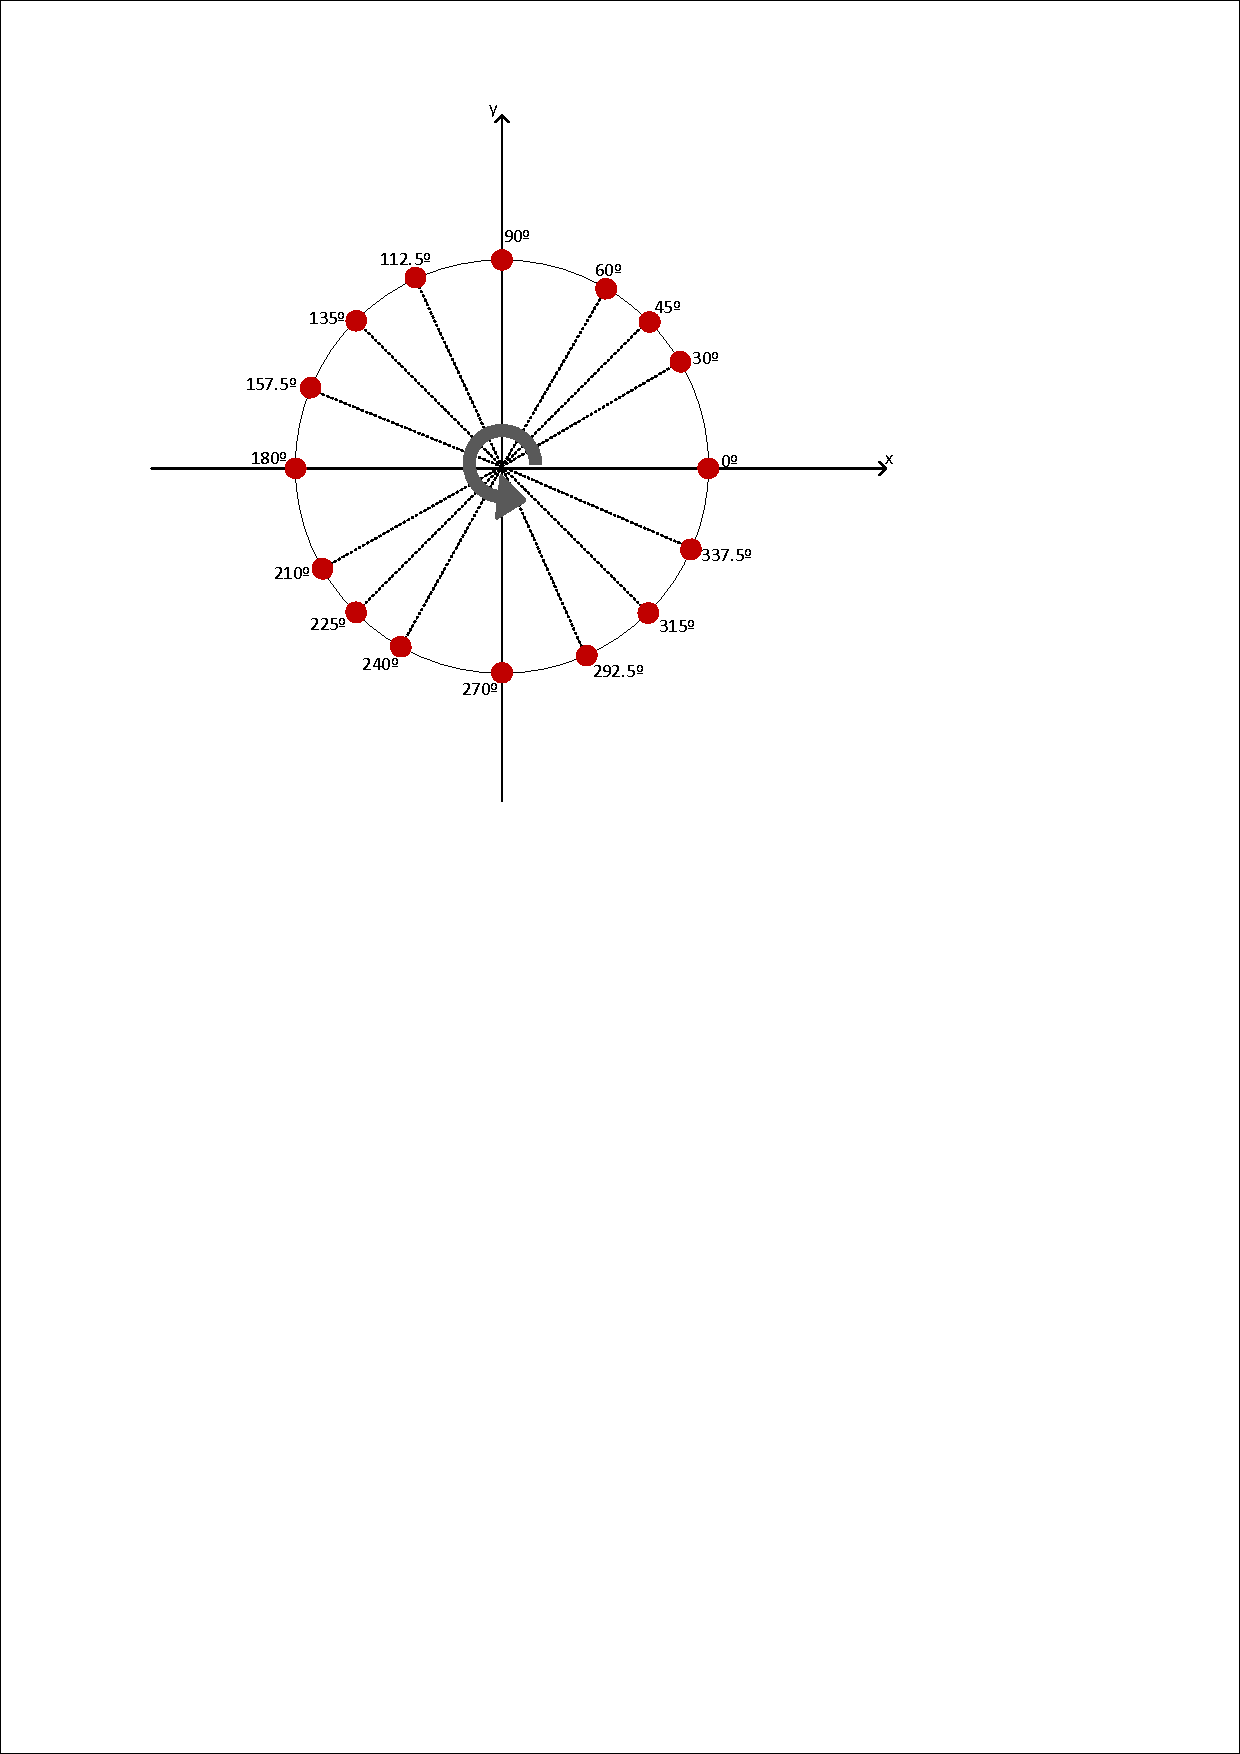
\includegraphics[clip, trim=0.5cm 15.5cm 2.5cm 1cm, height = 10cm]{./sdf/quantum_random_number_generator/figures/sphere.pdf}
    \caption{Angles used to perform the qrng simulation for $N=1 \times 10^{6}$ samples. }\label{sphere}
\end{figure}

For a quantum random number generator with equal probability of obtain a "0" \space or "1" \space the polarizer must be set at $45^{\circ}$. This way, we have $50\%$ possibilities to obtain a "0" \space and $50\%$ of possibilities to obtain a "1" \space. This theoretical value meets the value obtained from the simulation when it is performed for the number of samples mentioned above.

\begin{figure}[H]
    \centering
        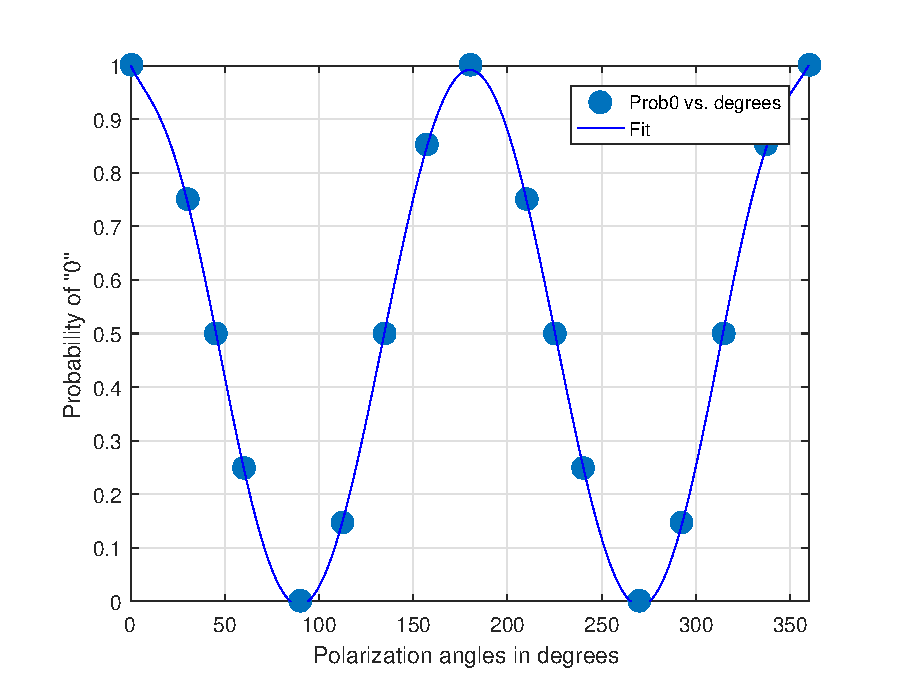
\includegraphics[width=15cm,height=10cm]{./sdf/quantum_random_number_generator/figures/prob0.eps}
    \caption{Probability of outputs a number "0" \space depending on the polarization angle.}\label{probx}
\end{figure}

Figure \ref{probx} shows the probability of a single photons reaches the detector placed on Horizontal axis depending on the polarization angle of the photon, and this way the output number is "0". The following table shows the goodness of the fit:
\begin{table}[H]
\centering
\label{tab:goodnessfitprob0}
    \begin{tabular}{c|c}
      SSE:                  & 0.0004785\\
      R-square:             &0.9998\\
      Adjusted R-square:    &0.9995\\
      RMSE:                 &0.007734
  \end{tabular}
\end{table}

On the other hand, figure \ref{proby} shows the probability of a single photon reaches the detector placed on Vertical component of the polarization beam splitter, and this way the output number is "1". As we can see in the figures the two detectors have complementary probabilities, i.e the summation of both values must be equals to $1$. One can see that "Probability of $1$" \space behaves almost like a sine function and "Probability of 0" \space behaves almost like a cosine function with a variable angle.

\begin{figure}[H]
    \centering
        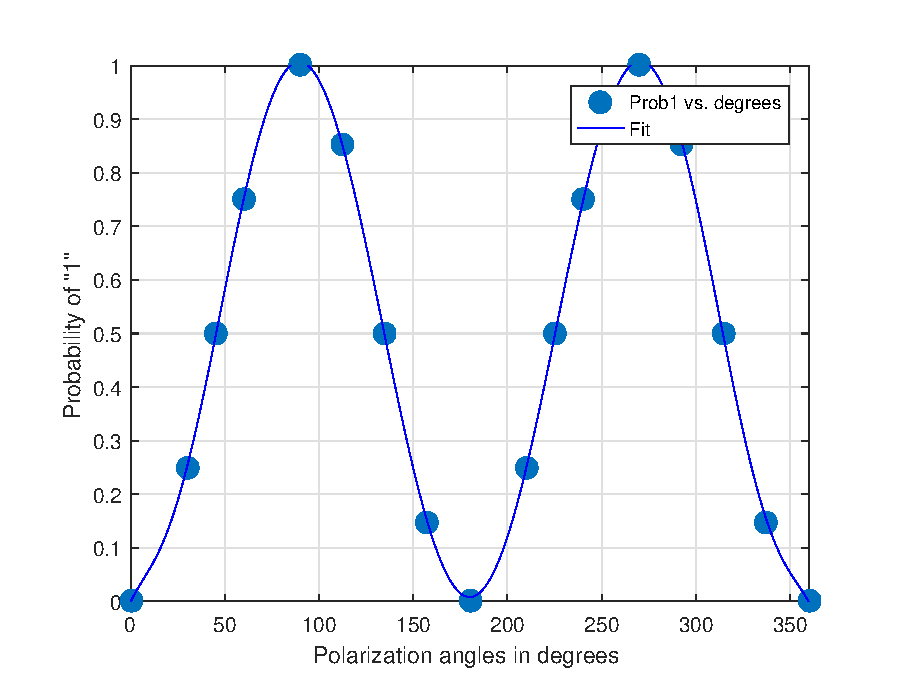
\includegraphics[width=15cm,height=10cm]{./sdf/quantum_random_number_generator/figures/prob1.eps}
    \caption{Probability of outputs a number "1" \space depending on the polarization angle.}\label{proby}
\end{figure}

The goodness of the fit presented in figure \ref{proby} is shown in the following table:
\begin{table}[H]
\centering
\label{tab:goodnessfitprob0}
    \begin{tabular}{c|c}
        SSE:                &0.0004785\\
        R-square:           &0.9998\\
        Adjusted R-square:  &0.9995\\
        RMSE:               &0.007734
  \end{tabular}
\end{table}

The goodness of the fit is evaluated based on four parameters:
\begin{enumerate}
  \item The sum of squares due to error (SSE), which measures the total deviation between the fit values and the values that the simulation outputs. This value is calculated from the expression
      \begin{equation}\label{}
        \textrm{SSE} = \sum_{i=1}^{n} w_i(y_{i}-\hat{y_{i}})^2.
        \nonumber
      \end{equation}
      A value of SSE closer to 0 means that the model has a small random error component.

  \item The R-square measures how good the fit in explaining the data.
    \begin{equation}\label{}
    \textrm{R-square} = 1-\frac{\textrm{SSE}}{\textrm{SST}},
    \nonumber
    \end{equation}
    where,
    \begin{equation}\label{}
    \textrm{SST} = \sum_{i=1}^{n} w_i (y_i - \bar{y_i})^2.
      \nonumber
    \end{equation}
    R-square can take a value between 0 and 1. If the value is closer to 1, it means that the fit better explains the total variation in the data around the average.

  \item Degrees of freedom adjusted R-square uses the R-square and adjusts it based on the number of degrees of freedom.
    \begin{equation}\label{}
      \textrm{adjusted R-square} = 1 - \frac{\textrm{SSE}(n-1)}{\textrm{SST}(v)},
      \nonumber
    \end{equation}
    where,
    \begin{equation}\label{}
      v = n - m,
      \nonumber
    \end{equation}
    where n is the number of values in test and m is the number of fitted coefficients estimated from the values in test. A value of adjusted R-square close to 1 is a indicative factor of a good fit.

  \item The root mean square error (RMSE) is also a fit standard error and it can be calculated from:
    \begin{equation}\label{}
      \textrm{RMSE} = \sqrt{\textrm{MSE}},
      \nonumber
    \end{equation}
    where,
    \begin{equation}\label{}
      \textrm{MSE} = \frac{\textrm{SSE}}{v}.
      \nonumber
    \end{equation}

\end{enumerate}

\subsection{Experimental Analysis}

In order to have a real experimental quantum random number generator, a setup shown in figure \ref{experimental_qrng} was built in the lab. To simulate a single photon source we have a CW-Pump laser with $1550$ nm wavelength followed by an interferometer Mach-Zenhder in order to have a pulsed beam. The interferometer has an input signal given by a Pulse Pattern Generator. This device also gives a clock signal for the Single Photon Detector (APD-Avalanche Photodiode) which sets the time during which the window of the detector is open. After the MZM there is a Variable Optical Attenuator (VOA) which reduces the amplitude of each pulse until the probability of one photon per pulse is achieved. Next, there is a polarizer controller followed by a Linear Polarized, which is set at $45^{\circ}$, then a Polarization Beam Splitter (PBS) and finally, one detector at the end of each output of the PBS. The output signals from the detector will be received by a Processing Unit. Regarding to acquired the output of the detectors, there is an oscilloscope capable of record $1 \times 10^{6}$ samples.



\begin{figure}[H]
    \centering
        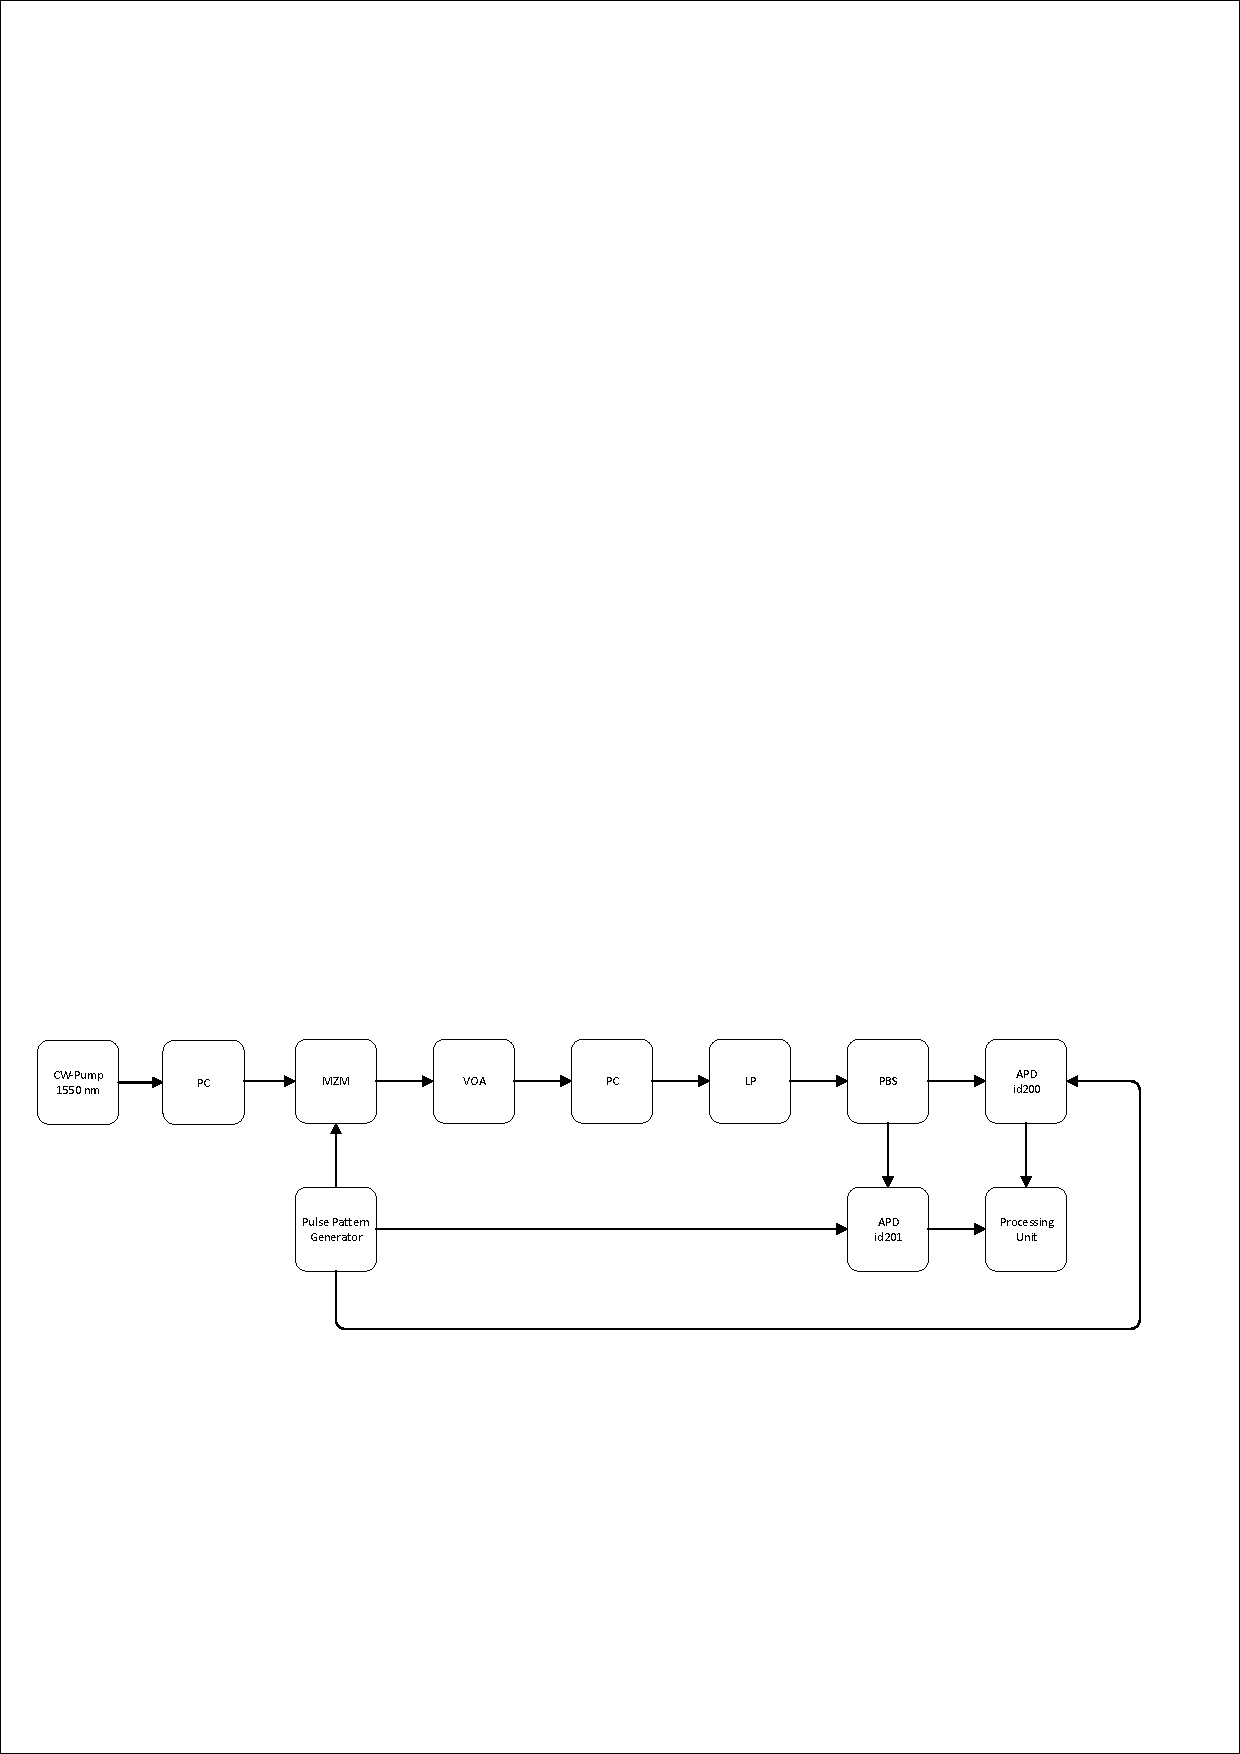
\includegraphics[clip, trim=0.5cm 7cm 0.5cm 17cm, width=1.00\textwidth]{./sdf/quantum_random_number_generator/figures/experimental_qrng.pdf}
    \caption{Experimental setup to implement a quantum random number generator.}\label{experimental_qrng}
\end{figure}

\subsubsection{IDQuantique detector}
%
The detector used in the laboratory is the Thorlabs PDB 450C. This detector consists of two well-matched photodiodes and a transimpedance amplifier that generates an output voltage (RF OUTPUT) proportional to the difference between the photocurrents of the photodiodes.\\
Additionally, the unit has two monitor outputs (MONITOR+ and MONITOR-) to observe the optical input power level on each photodiode separately.

Since we do not have a single photon source, we must use the Poisson Statistics in order to calculate the best value for a mean of photons per pulse. A weak laser pulse follows a Poissonian Statistics\cite{markfox}:
\begin{equation}\label{eq:poisson}
  S_n = e^{-\mu}\frac{\mu^{n}}{n!},
\end{equation}
where $\mu$ is the average photon number. In addition, the probability of an optical pulse carries one photon at least is:
\begin{equation}\label{eq:prob1photon}
  P = 1 - S_0 = 1 - e^{-\mu}.
\end{equation}

On the other hand, the probability of a detector clicks is:

\begin{equation}\label{eq:detectorclickprob}
  P_{click} = P_{det}+P_{dc} + P_{det}P_{dc},
\end{equation}

where $P_{det}$ is the probability of the detector clicks due a photon which cross its window and $P_{dc}$ is the probability of dark counts. Considering the detector efficiency $\eta_{D}$, the probability of the detector clicks due to a photon is:

\begin{equation}\label{eq:probclickefficiency}
  P_{det} = 1 - e^{- \eta_{D}\mu}.
\end{equation}

The probability of dark counts is calculated as a ratio between the frequency counts and the trigger frequency when no laser is connected to the detector. Nevertheless, the detector click frequency is
\begin{equation}\label{eq:frequencyclick}
  f_{click} = f_{trigger}P_{click} \longrightarrow P_{click}=\frac{f_{click}}{f_{trigger}}.
\end{equation}

This way the mean average photon number can be calculate using the following equation:
\begin{equation}\label{eq:meanphotonnumber}
  \mu = - \frac{1}{\eta_{D}}\ln\left [1-\frac{1}{1-P_{dc}}\left (\frac{f_{click}}{f_{trigger}}-P_{dc} \right)\right]
\end{equation}

\subsection{Open Issues}

\newpage


%%%%%%%%%%%%%%%%%%%%%%%%%%%%%%%%%%%%%%%%%%%%%%%%%%%%%%%%%%%%%%%%%%%%%%%%%%%%%%%%%%%%%%%%%%%%%%%%%%%%%%%%%%%%
% References
%%%%%%%%%%%%%%%%%%%%%%%%%%%%%%%%%%%%%%%%%%%%%%%%%%%%%%%%%%%%%%%%%%%%%%%%%%%%%%%%%%%%%%%%%%%%%%%%%%%%%%%%%%%%

\renewcommand{\bibname}{References}
%
\bibliographystyle{myIEEEtran}
% argument is your BibTeX string definitions and bibliography database(s)
\bibliography{./sdf/quantum_random_number_generator/quantum_random_number_generator}
%
%


\cleardoublepage
